\paragraph{}
        Le projet PFA a pour objectif de faire découvrir aux élèves la gestion d'un projet depuis la création du cahier des charges jusqu'à l'implémentation en ayant affaire à des clients réels. C'est le premier projet du cursus se réalisant avec un groupe de taille conséquente (en moyenne 7 personnes) et dans lequel les élèves établissent les spécifications du rendu en échangeant avec le client. Le travail se décompose en deux phases : une première phase durant le premier semestre pour établir les besoins, et les présenter de manière formelle dans le cahier des charges, puis une deuxième phase au cours du second semestre pour concrétiser ces besoins en réalisant ce qui est spécifié.

\paragraph{}      
        Le projet PFA effectué : De la 3D à la 2D, est un projet d'imagerie numérique. L'objectif est de réaliser une scène 3D constituée de un ou plusieurs modèles 3D pour ensuite générer des vues en deux dimensions de celle-ci, comme présentée dans la figure \ref{fig:3Don}. Ces dernières seront utilisées pour obtenir une illusion en trois dimensions en se basant sur des principes connus. Les algorithmes étudiés au cours de ce projet permettent de générer des anaglyphes, autostéréogrammes et folioscopes, également appelés flipbooks,  qui seront présentés plus en détails dans la suite du rapport.
        
\paragraph{}
        Dans ce rapport, nous présenterons dans un premier temps le domaine de la synthèse d'image, les rendus à implémenter dans notre logiciel et les objectifs donnés dans le cahier des charges. Nous parlerons ensuite de la réalisation technique de notre logiciel, depuis les choix effectués pour la programmation et les algorithmes jusqu'au déroulement du projet et aux difficultés rencontrées. Enfin, nous ferons un bilan de cet expérience de gestion de projet, depuis la phase de cahier des charges jusqu'au rendu.

\begin{figure}[h]
	\centering
	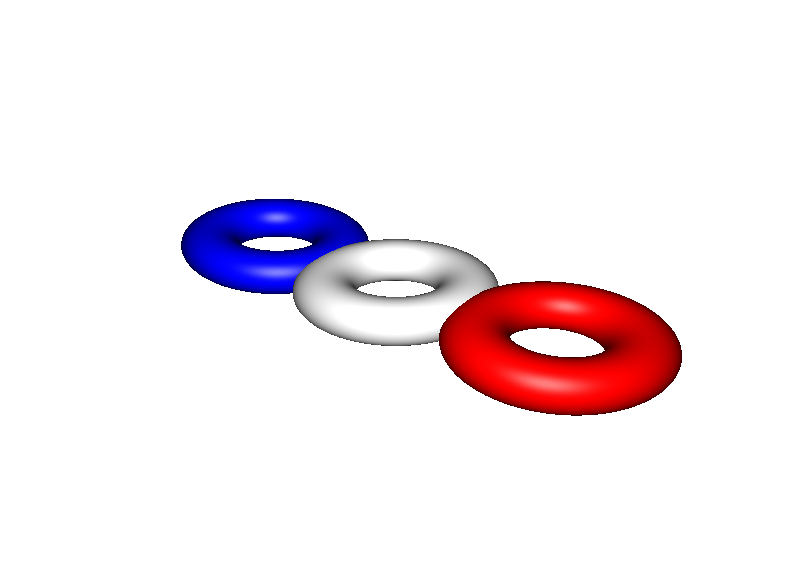
\includegraphics[scale=0.4]{3donut_rendu.png}
	\caption{\label{fig:3Don} Rendu classique du projet \protect}
\end{figure}
